%%%%%%%%%%%%%%%%%%%%%%%%%%%%%%%%%%%%%%%%%
% Beamer Presentation
% LaTeX Template
% Version 1.0 (10/11/12)
%
% This template has been downloaded from:
% http://www.LaTeXTemplates.com
%
% License:
% CC BY-NC-SA 3.0 (http://creativecommons.org/licenses/by-nc-sa/3.0/)
%
%%%%%%%%%%%%%%%%%%%%%%%%%%%%%%%%%%%%%%%%%

%----------------------------------------------------------------------------------------
%	PACKAGES AND THEMES
%----------------------------------------------------------------------------------------

\documentclass{beamer}

\mode<presentation> {

% The Beamer class comes with a number of default slide themes
% which change the colors and layouts of slides. Below this is a list
% of all the themes, uncomment each in turn to see what they look like.

%\usetheme{default}
%\usetheme{AnnArbor}
%\usetheme{Antibes}
%\usetheme{Bergen}
%\usetheme{Berkeley}
%\usetheme{Berlin}
%\usetheme{Boadilla}
%\usetheme{CambridgeUS}
%\usetheme{Copenhagen}
%\usetheme{Darmstadt}
%\usetheme{Dresden}
%\usetheme{Frankfurt}
%\usetheme{Goettingen}
%\usetheme{Hannover}
%\usetheme{Ilmenau}
%\usetheme{JuanLesPins}
%\usetheme{Luebeck}
\usetheme{Madrid}
%\usetheme{Malmoe}
%\usetheme{Marburg}
%\usetheme{Montpellier}
%\usetheme{PaloAlto}
%\usetheme{Pittsburgh}
%\usetheme{Rochester}
%\usetheme{Singapore}
%\usetheme{Szeged}
%\usetheme{Warsaw}

% As well as themes, the Beamer class has a number of color themes
% for any slide theme. Uncomment each of these in turn to see how it
% changes the colors of your current slide theme.

%\usecolortheme{albatross}
%\usecolortheme{beaver}
%\usecolortheme{beetle}
%\usecolortheme{crane}
%\usecolortheme{dolphin}
%\usecolortheme{dove}
%\usecolortheme{fly}
%\usecolortheme{lily}
%\usecolortheme{orchid}
%\usecolortheme{rose}
%\usecolortheme{seagull}
%\usecolortheme{seahorse}
%\usecolortheme{whale}
%\usecolortheme{wolverine}

%\setbeamertemplate{footline} % To remove the footer line in all slides uncomment this line
\setbeamertemplate{footline}[page number] % To replace the footer line in all slides with a simple slide count uncomment this line

%\setbeamertemplate{navigation symbols}{} % To remove the navigation symbols from the bottom of all slides uncomment this line
}

\usepackage{graphicx} % Allows including images
\usepackage{booktabs} % Allows the use of \toprule, \midrule and \bottomrule in tables
\usepackage{xcolor}% or package color
\usepackage{amssymb}
\usepackage{amsmath}
\usepackage{bm}
\usepackage{mathtools}
\usepackage{tikz}
\usetikzlibrary{trees}
\usetikzlibrary{arrows.meta, bending}
\usepackage[percent]{overpic}
\usepackage{pdfpages}

\graphicspath{{./Figures/}}

%----------------------------------------------------------------------------------------
%	TITLE PAGE
%----------------------------------------------------------------------------------------

\title[lab meeting]{Genetic rescue by introgressive hybridization} % The short title appears at the bottom of every slide, the full title is only on the title page

\author{F.J.H. de Haas \& S.P. Otto} % Your name

\date{\today} % Date, can be changed to a custom date

\begin{document}

\begin{frame}
\titlepage % Print the title page as the first slide
\end{frame}

\begin{frame}{Orr and Unckles 2014}

Evolutionary rescue is characterized by a U-shaped curve of population size.

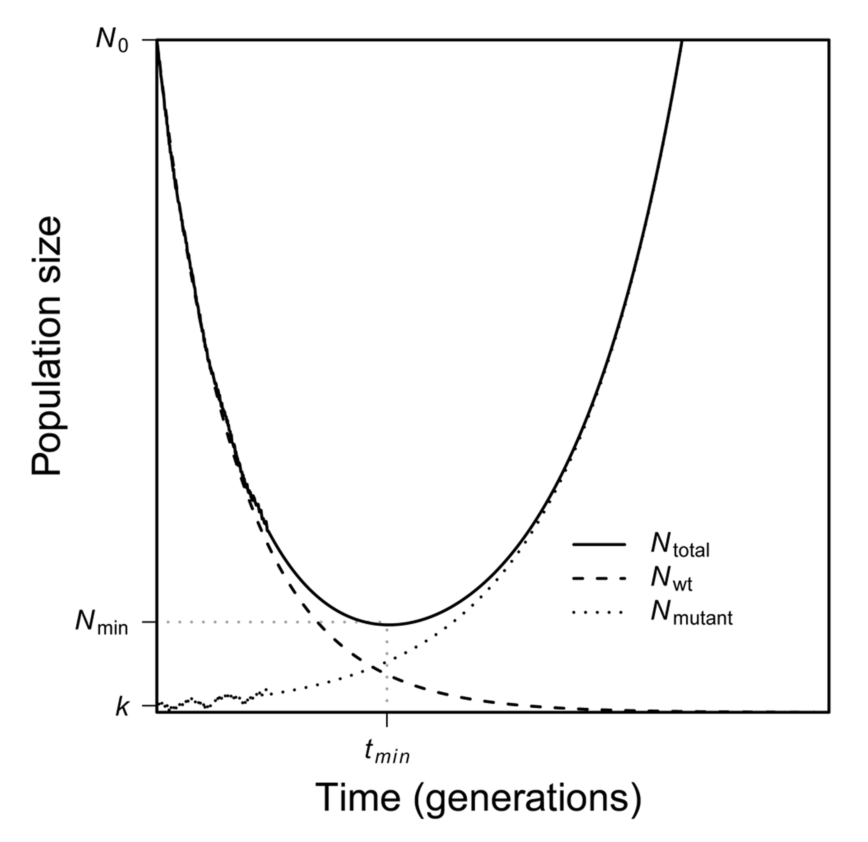
\includegraphics[width=0.5\columnwidth]{Ushape_ER.png}

We look at \textcolor{red}{genetic rescue} conditioned on evolutionary rescue.

\end{frame}

\begin{frame}{Genetic rescue}
    What is \textcolor{red}{genetic rescue}? Some general explanation what we understand by genetic rescue. use recombination
\end{frame}

\begin{frame}{Overview}
    Introduce the different techniques to get at the question: analytical approach, markov approach, simulations. Prep the minds. Mention that all model outcome of genetic rescue condition on fixation.
\end{frame}

\begin{frame}{The 2 locus model}

\begin{center}
\begin{tabular}{ c | c c c c}
 Genotype & AB & Ab & aB & ab\\ 
  \hline
 Frequency & p_nQ_n & p_n(1-Q_n) & (1-p_n)R_n & (1-p_n)(1-R_n)\\  
 Fitness & 1+s & 1+s & 1 & 1   
\end{tabular}
\end{center}

Assume a wildtype population of $aB$ haplotypes and a few introduced $Ab$ rescue haplotypes. 

\textcolor{red}{Genetic rescue} is defined:
\begin{equation*}
    \lim_{n\to\infty} \frac{AB_n}{AB_n+Ab_n} = \lim_{n\to\infty} \frac{p_nQ_n}{p_nQ_n+p_n(1-Q_n)} = \lim_{n\to\infty} Q_n
\end{equation*}

When $Q_0 = 0$, $R_0 = 1$ and $r=0.5$, a recursion equation for $Q_n$ is derived: 

\begin{equation*}
    \color{red} Q_n = \sum_{i=1}^n 2^{-i} (1-p_i)
\end{equation*}

\end{frame}

\begin{frame}{Numerical Simulation}
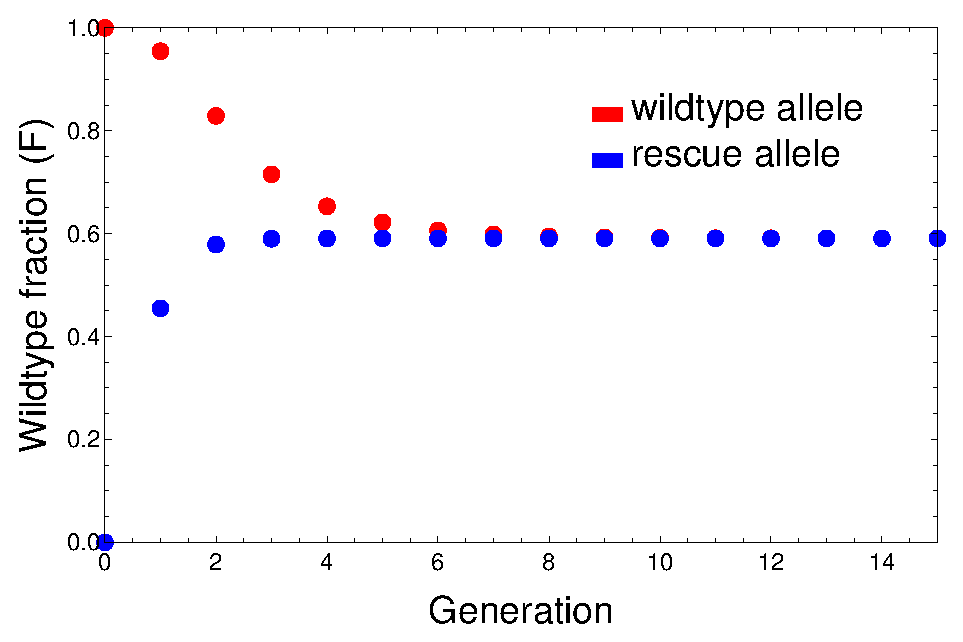
\includegraphics[width=0.9\textwidth]{Figures/NumericalSolution.eps}

\end{frame}

\begin{frame}{The infinite loci model}

\begin{equation}
    \begin{array}{l}
	F_w[t+1] = \overbrace{\frac{1}{2} (F_w[t]+F_b[t]) p_b[t+1]}^\text{$w$ x $b$}  + \overbrace{F_w[t] (1-p_b[t+1])}^\text{$w$ x $w$}
	 \\ \\
	F_b[t+1]  = \overbrace{\frac{1}{2} (F_w[t]+F_b[t]) (1-p_b[t+1])}^\text{$b$ x $w$} 
	+ \overbrace{F_b[t] p_b[t+1]}^\text{$b$ x $b$}
	\end{array}
\end{equation}

Assumptions: \\
1) Infinite population size \\
2) Infinite \# of loci \\
3) Free recombining loci ($r = 0.5$) 
    
\begin{equation*}
    \color{red} F_b[t] = \sum_{i=1}^t 2^{-t} (1-p_t)
\end{equation*}
\end{frame}

\begin{frame}{Discrete markov birth-death model}
\footnotesize

$\bold{P} = \{\{G_{AB},G_{Ab},G_{aB},G_{ab}\}\} \text{ such that } G_i\in\{0,1,...,n\}$\\ 
$\bold{X},\bold{Y} \in \bold{P}$. \\

Probability of going from $\bold{X}$ to $\bold{Y}$
\begin{equation*}
\bold{M}_{\bold{Y},\bold{X}}=
\begin{aligned}
\begin{cases}
\begin{cases}
    p_{AB+1}, & \text{if } \bold{Y} = \bold{X} + \{1,0,0,0\}; \\
    p_{Ab+1}, & \text{if } \bold{Y} = \bold{X} + \{0,1,0,0\};  \\
    p_{aB+1}, & \text{if } \bold{Y} = \bold{X} + \{0,0,1,0\}; \\
    p_{ab+1}, & \text{if } \bold{Y} = \bold{X} + \{0,0,0,1\}; \\
    p_{AB-1}, & \text{if } \bold{Y} = \bold{X} + \{-1,0,0,0\}; \\
    p_{Ab-1}, & \text{if } \bold{Y} = \bold{X} + \{0,-1,0,0\};  \\
    p_{aB-1}, & \text{if } \bold{Y} = \bold{X} + \{0,0,-1,0\}; \\
    p_{ab-1}, & \text{if } \bold{Y} = \bold{X} + \{0,0,0,-1\}; \\
    1, & \text{if}\ \bold{X} = \bold{Y} = \{0,0,0,0\}; \\
    0, & otherwise;
\end{cases}  & \text{if}\ \bold{X}_1, \bold{X}_2 \neq n; \\
\begin{cases} 
    1, & \text{if}\ \bold{X}_1 = \bold{Y}_1 = n; \\
    1, & \text{if}\ \bold{X}_2 = \bold{Y}_2 = n;  \\
    \mathrlap{0,}\hphantom{p_{AB+1},} & otherwise;
\end{cases} & otherwise;
\end{cases},
\end{aligned}
\end{equation*}
\normalsize

\end{frame}

\begin{frame}{Probabilites of birth-death model}

\footnotesize
Each type has a birth- and death-rate $b_i$ and $d_i$ respectively. Selection is implemented in the death rates. All types have the same birthrate $b_{AB}=b_{Ab}=b_{aB}=b_{ab} =1$  

    \begin{equation*}
    \begin{aligned}
        P_{i|\text{death}}=\frac{f_id_i}{\sum_{i=1}^4 f_id_i} \qquad P_\text{birth} = \frac{\sum_i^4 f_i b_i}{\sum_i^4 (f_i b_i + f_i d_i)} 
    \end{aligned}
    \end{equation*}
    
    \begin{equation*}
    \begin{aligned}
        &p_{AB+1} & =& (f_{AB}-r\times D) & \times P_\text{birth};\\
        &p_{Ab+1} & =& (f_{Ab}+r\times D) & \times P_\text{birth};\\
        &p_{aB+1} & =& (f_{aB}+r\times D) & \times P_\text{birth};\\
        &p_{ab+1} & =& (f_{ab}-r\times D) & \times P_\text{birth};\\
        &p_{AB-1} & =& P_{AB|\text{death}} & \times (1-P_\text{birth}); \\
        &p_{Ab-1} & =& P_{Ab|\text{death}} & \times (1-P_\text{birth}); \\
        &p_{aB-1} & =& P_{aB|\text{death}} & \times (1-P_\text{birth}); \\
        &p_{ab-1} & =& P_{ab|\text{death}} & \times (1-P_\text{birth}); 
    \end{aligned}
    \end{equation*} 

    
 \normalsize
    
\end{frame}

\begin{frame}{Example of absorbing states}
    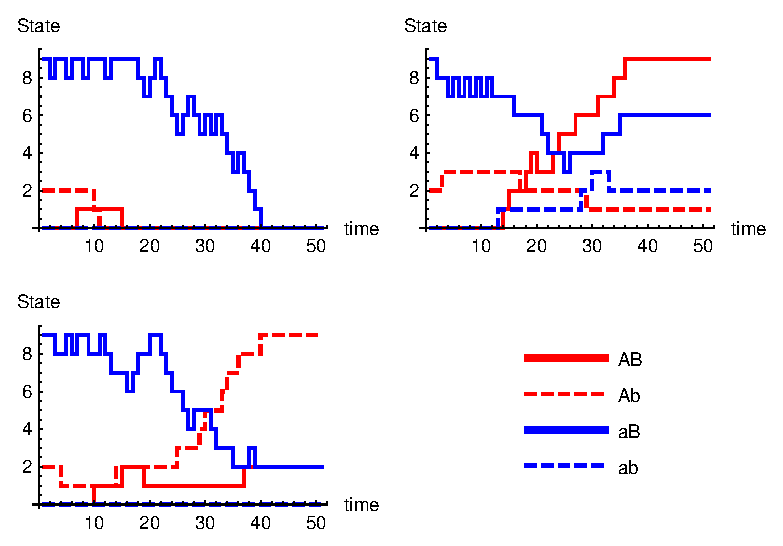
\includegraphics[width=1.0\textwidth]{Matlab/Figures/gridplot.eps}
\end{frame}



\begin{frame}{$F_A$ from process $\bold{X}(t)$.}
    
    $P[\bold{X}(\infty) = \bold{A}| \bold{X}(0) = \bold{I}]$ satisfies the left eigenvector $p_\bold{A}^\intercal$ with $\lambda = 1$ and the corresponding right eigenvector $=\bold{A}$:
    
    \begin{equation*}
        \vec{p}_\bold{A}^\intercal = \vec{p}_\bold{A}^\intercal \bold{M} \ \ \ \  \text{subject to } p_{\bold{A},\bold{A}}=1 \ \text{and}\ p_{l,\bold{A}}=0
    \end{equation*}.
    
    The expected deterministic projection can be calculated from the probabilities of getting absorbed: 
    
    \begin{equation*}
        \mathbb{E}[F(\bold{I})] = \vec{p}_\bold{A}(\bold{I}) \bullet \vec{F}_A   %transpose and do dot product with 
    \end{equation*}
    
    where $\vec{F}_A$ is a vector containing the deterministic projections for each absorbing state. (*Need to specify we drop the {0,0,0,0} case*)
\end{frame}

\begin{frame}{Numerical simulation}
    $r=0.5$,  $W_A=1.1$ and $W_a=0.9$.
    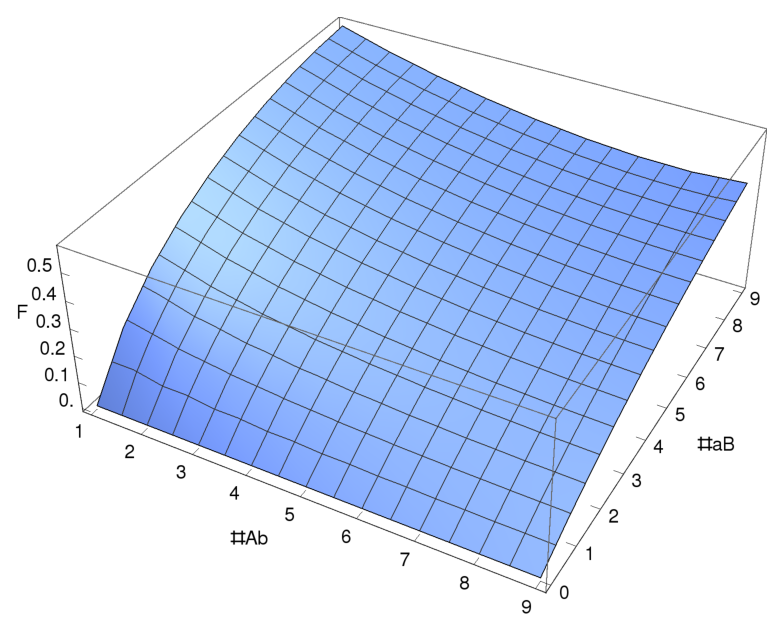
\includegraphics[width=0.75\textwidth]{Matlab/Figures/Projection3DPlotr050.eps}
\end{frame}

\begin{frame}{Comparing model outcomes}

\begin{tabular}{l | l | lll | lll}  
&  & \multicolumn{6}{c}{$W_A=1.1$ and $W_a = 0.9$}
&  & \multicolumn{3}{c}{$r=0.5$} & \multicolumn{3}{c}{$r=0.05$} \\
\midrule
$Ab$& $aB$ & Det & Stoch & Sim & Det & Stoch & Sim \\
\midrule
1 & 1 & 0.404 & 0.184 &          & 0.113 & 0.033 & \\
     & 5 & 0.767 & 0.495 &          & 0.256 & 0.103 &  \\
     & 9 & 0.854 & 0.583 &          & 0.302 & 0.126 &  \\
     \midrule
5 & 1 & 0.121 & 0.092 &          & 0.031 & 0.021 &  \\
     & 5 & 0.404 & 0.328 &          & 0.113 & 0.081 &  \\
     & 9 & 0.547 & 0.425 &           & 0.162 & 0.106 & \\
     \midrule
9 & 1 & 0.071 & 0.071 &          & 0.018 & 0.018 &  \\
     & 5 & 0.275 & 0.275 &          & 0.073 & 0.073 &  \\
     & 9 & 0.404 & 0.404 &           & 0.113 & 0.113 & \\
\end{tabular}
\end{frame}



\begin{frame}{Individual based simulations}
    
    An individual contains a genome with multiple loci. Simulations are conditioned on fixation.
    
    \vfill

    \begin{minipage}{0.45\textwidth}
    \begin{itemize}
      \item Birth \\
          \begin{itemize}
          \item{Poisson with  $\lambda \approx b$}
          \item{Choose random mate}
        \end{itemize}
      \item Death \\
      \begin{itemize}
          \item $\textit{U}(0,1) < d_i$
      \end{itemize}
    \end{itemize}
    \end{minipage}%
    \hfill
    \begin{minipage}{0.45\textwidth}
    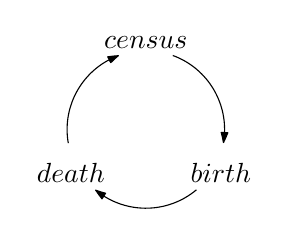
\begin{tikzpicture}[-{Stealth[inset=0pt,length=4.5pt,angle'=35,round,bend]}, scale=1]
      \foreach \a/\t in {90/census,-30/birth,210/death}{
        \node (\t) at (\a:1.1cm) {$\t$};
        \draw (\a-20:1cm)  arc (\a-20:\a-100:1cm);
      } 
    \end{tikzpicture}
    \end{minipage}%


\end{frame}


\begin{frame}{Comparing model outcomes}

\begin{tabular}{l | l | lll | lll}
&  & \multicolumn{6}{c}{$W_A=1.1$ and $W_a = 0.9$}
&  & \multicolumn{3}{c}{r=0.5} & \multicolumn{3}{c}{r=0.05} \\
\midrule
Ab& aB & Det & Stoch & Sim & Det & Stoch & Sim \\
\midrule
1 & 1 & 0.404 & 0.184 & 0.35         & 0.113 & 0.033 & 0.302 \\
     & 5 & 0.767 & 0.495 & 0.699           & 0.256 & 0.103 & 0.629  \\
     & 9 & 0.854 & 0.583 & 0.803         & 0.302 & 0.126 &  0.726\\
     \midrule
5 & 1 & 0.121 & 0.092 &  0.137         & 0.031 & 0.021 & 0.189 \\
     & 5 & 0.404 & 0.328 & 0.429          & 0.113 & 0.081 & 0.402\\
     & 9 & 0.547 & 0.425 & 0.565          & 0.162 & 0.106 & 0.531 \\
     \midrule
9 & 1 & 0.071 & 0.071 & 0.092         & 0.018 & 0.018 & 0.073\\
     & 5 & 0.275 & 0.275 & 0.309          & 0.073 & 0.073 &  \\
     & 9 & 0.404 & 0.404 & 0.440           & 0.113 & 0.113 & \\
\end{tabular}
\end{frame}

\begin{frame}{Expand simulations to loci with local adaptation and non-random mating}
    
\end{frame}

\begin{frame}{Slide Graveyard}


    \begin{equation*}
    \begin{aligned}
        f_{AB}(t+1)= &(f_{AB}(t)^2(1+s)^2+f_{AB}f_{aB}(1+s)+f_{AB}f_{Ab}(1+s)^2+ \\
        &f_{AB}f_{ab}(1+s)(1-r)+f_{aB}f_{Ab}(1+s)r)/(\bar{W}^2) \\
        f_{Ab}(t+1)=    \\
        f_{aB}(t+1)=    \\
        f_{ab}(t+1)=
        \end{aligned}
    \end{equation*}
    
\begin{equation*}
    F_A(t)= \frac{f_{AB}(t)}{f_{AB}(t)+f_{Ab}(t)}
\end{equation*}

$F_A$ represents the proportion of $B$ alleles that have been rescued because they have recombined to a $A$ rescue allele.



\end{frame}

\end{document}